%% ---- DOCUMENT CLASS
%% -------- Tamano hoja: A4, tamano fuente cuerpo texto: 11 pt, clase de documento: book, formato hoja: doble faz (twoside) 
\documentclass[a4paper, 11pt, twoside]{book}

\raggedbottom

%% ---- ARCHIVO DE ESTILOS
%% -------- Resto de configuraciones de formato se define en el archivo *formato_PI.sty*
\usepackage{formato_PI}


%% ---- PARTES DEL DOCUMENTO

\begin{document}


    \frontmatter

    \pagenumbering{roman}

    %--------------------------------------------------------------------------------------------------------------------------
    %  PORTADA
    %--------------------------------------------------------------------------------------------------------------------------
    \begin{titlepage}
    \centering
    {
\includegraphics[width=0.225\textwidth]{../img/logo.jpg}}
    \hspace{1cm}
    {
\includegraphics[width=0.15\textwidth]{../img/fcefyn.png}\par}
    \vspace{1cm}
    {\bfseries\LARGE Universidad Nacional de Córdoba \par}
    \vspace{0.7cm}
    {\scshape\Large Facultad de Ciencias Exactas, Físicas y Naturales\par}
    \vspace{2cm}
    {\scshape\Huge Compiladores y ejecutables \par}
    \vspace{2cm}
    {\itshape\Large Práctica Supervisada \par}
    \vspace{1.5cm}
    {\itshape\large Informe de Trabajo \par}
    \vfill
    \vspace{0.5cm}
    {\Large Supervisor: \par}
    \vspace{0.3cm}
    {\Large \textbf{Prof. Maximiliano Eschoyez}\par}
    \vspace{0.5cm}
    {\Large Tutor: \par}
    \vspace{0.3cm}
    {\Large \textbf{Nicolás Papp}\par}
    \vspace{0.5cm}
    {\Large Autores: \par}
    \vspace{0.3cm}
    {\Large \textbf{\emph{José Cancinos}} y \textbf{\emph{Julián González}}\par}
    \vfill
    \vspace{0.5cm} 
    {\small 2021 \par}
\end{titlepage}



    %--------------------------------------------------------------------------------------------------------------------------
    %  ACTA DE EXAMEN
    %--------------------------------------------------------------------------------------------------------------------------
    \chapter*{}
\begin{center}
	
	% Logo universidad
	\begin{figure}[h]
		\begin{center}
			
\includegraphics[scale=0.8]{logo_unc.png}
		\end{center}
	\end{figure}
	\vspace{0.25em}
	
	\textsc{\LARGE Universidad Nacional de Córdoba}\\[0.3cm] % Name of your university/college
	\textsc{\large Facultad de Ciencias Exactas, Físicas y Naturales}\\[0.3cm] % Major heading such as course name
	\textsc{\large Escuela de Ingeniería Electrónica}\\[0.75cm] % Minor heading such as course title
\end{center}


El Tribunal Evaluador reunido en este acto y luego de haber aprobado la Solicitud de Aprobación de Tema 
y efectuado las distintas instancias de correcciones del Informe del Proyecto Integrador para la obtención 
del Título de Grado “Ingeniero Electrónico” y cumpliendo con el Reglamento correspondiente, declaran el Informe 
Final de los estudiantes \textbf{Apellido, Nombres} y \textbf{Apellido, Nombres} como “aceptado sin correcciones” 
y la defensa oral Aprobada. Por lo tanto, luego de haber tenido en cuenta los aspectos de evaluación que indica el 
Reglamento, el Proyecto Integrador se considera Aprobado. 

\vspace{0.5cm}

\par Se firma el Acta de Examen correspondiente y se distribuyen los ejemplares impresos.

\vspace{4.5cm}

Firma y aclaración del Tribunal Evaluador:

\vspace{0.5cm}

Fecha:

\clearpage{\thispagestyle{empty}\cleardoublepage}       %% Comando para insertar pagina en blanco al ser doble pagina y remover fancy headers

    %--------------------------------------------------------------------------------------------------------------------------
    %  ACTA DEFENSA
    %--------------------------------------------------------------------------------------------------------------------------
    \chapter*{}
\begin{center}
	
	% Logo universidad
	\begin{figure}[h]
		\begin{center}
			
\includegraphics[scale=0.8]{logo_unc.png}
		\end{center}
	\end{figure}
	\vspace{0.25em}
	
	\textsc{\LARGE Universidad Nacional de Córdoba}\\[0.3cm] % Name of your university/college
	\textsc{\large Facultad de Ciencias Exactas, Físicas y Naturales}\\[0.3cm] % Major heading such as course name
	\textsc{\large Escuela de Ingeniería en Computación}\\[0.75cm] % Minor heading such as course title
\end{center}

Quien suscribe el Profesor \textbf{Apellido, Nombres} en su carácter de Director del Proyecto Integrador de los 
Estudiantes: \textbf{Apellido, Nombres} y \textbf{Apellido, Nombres}, denominado \textbf{Título del proyecto integrador}, 
considera que el desarrollo del trabajo se ha completado según lo especificado en la Solicitud de Aprobación de Tema y 
se encuentra en condiciones de tramitar su defensa.

\begin{flushright}

    \vspace{1cm}

    A los efectos de quién corresponda, en fecha ……/……/……

    \vspace{4cm}

    Firma y aclaración del Director

\end{flushright}

\clearpage{\thispagestyle{empty}\cleardoublepage}       %% Comando para insertar pagina en blanco al ser doble pagina y remover fancy headers

    %--------------------------------------------------------------------------------------------------------------------------
    %  DEDICATORIA
    %--------------------------------------------------------------------------------------------------------------------------
    \chapter*{Dedicatoria}
\addcontentsline{toc}{chapter}{Dedicatoria}

\begin{flushright}
	\textit{Para nuestras familias...}
\end{flushright}

\clearpage{\thispagestyle{empty}\cleardoublepage}       %% Comando para insertar pagina en blanco al ser doble pagina y remover fancy headers

    %--------------------------------------------------------------------------------------------------------------------------
    %  AGRADECIMIENTOS
    %--------------------------------------------------------------------------------------------------------------------------
    \chapter*{Agradecimientos}
\addcontentsline{toc}{chapter}{Agradecimientos} 

\textit{A nuestros padres, madres y hermanos, por su incondicional apoyo a lo largo de toda la carrera.}

\vspace{1cm}

\textit{A nuestros directores, Apellido Nombre y Apellido Nombre, por la excelente predisposición, la confianza y todo el soporte brindado que hizo posible este proyecto.}

\vspace{1cm}

\textit{A nuestros amigos y futuros colegas, quienes hicieron de estos años de estudio una experiencia más placentera.}

\vspace{1cm}

\textit{A -Lugar donde se realizó el PI-, junto a todo su personal, por las oportunidades y enseñanzas compartidas.}

\vspace{1cm}

\textit{A la Facultad de Ciencias Exactas, Físicas y Naturales de la Universidad Nacional de Córdoba, por la oportunidad de realizar esta carrera de grado.}


\clearpage{\thispagestyle{empty}\cleardoublepage}       %% Comando para insertar pagina en blanco al ser doble pagina y remover fancy headers

    %--------------------------------------------------------------------------------------------------------------------------
    %  RESUMEN
    %--------------------------------------------------------------------------------------------------------------------------
    \chapter*{Resumen}
\addcontentsline{toc}{chapter}{Resumen}

En este trabajo...

%% -------------------------------------------
\vspace{4.5cm}  %% BORRAR AL COMPLETAR SECCION
%% -------------------------------------------

\textbf{Áreas Temáticas del Proyecto Integrador}: 

\textbf{Asignaturas}: 

\textbf{Palabras Claves}:

\clearpage{\thispagestyle{empty}\cleardoublepage}       %% Comando para insertar pagina en blanco al ser doble pagina y remover fancy headers

    %--------------------------------------------------------------------------------------------------------------------------
    %  ABSTRACT
    %--------------------------------------------------------------------------------------------------------------------------
    \chapter*{Abstract}
\addcontentsline{toc}{chapter}{Abstract}

In this thesis...

%% -------------------------------------------
\vspace{4.5cm}  %% BORRAR AL COMPLETAR SECCION
%% -------------------------------------------

\textbf{Key Words}: 

\clearpage{\thispagestyle{empty}\cleardoublepage}       %% Comando para insertar pagina en blanco al ser doble pagina y remover fancy headers






    

    %--------------------------------------------------------------------------------------------------------------------------
    % ÍNDICE
    %--------------------------------------------------------------------------------------------------------------------------
    \addcontentsline{toc}{chapter}{Índice}

\tableofcontents




    %--------------------------------------------------------------------------------------------------------------------------
    % LISTA DE FIGURAS
    % Incluir numero de figura, titulo de la figura y numero de pagina.
    %--------------------------------------------------------------------------------------------------------------------------
    \chapter*{Lista de Figuras}
\addcontentsline{toc}{chapter}{Lista de Figuras}

\listoffigures
\clearpage{\thispagestyle{empty}\cleardoublepage}       %% Comando para insertar pagina en blanco al ser doble pagina y remover fancy headers

    %--------------------------------------------------------------------------------------------------------------------------
    % LISTA DE TABLAS
    % Incluir numero de tabla, titulo de la tabla y numero de pagina.
    %--------------------------------------------------------------------------------------------------------------------------
    \chapter*{Lista de Tablas}
\addcontentsline{toc}{chapter}{Lista de Tablas}

\listoftables{}

\clearpage{\thispagestyle{empty}\cleardoublepage}       %% Comando para insertar pagina en blanco al ser doble pagina y remover fancy headers

    %--------------------------------------------------------------------------------------------------------------------------
    % LISTA DE CODIGOS
    % Incluir numero de listing de codigo, titulo de la listing y numero de pagina.
    %--------------------------------------------------------------------------------------------------------------------------
    \addcontentsline{toc}{chapter}{Lista de Códigos}
\renewcommand\lstlistlistingname{Lista de Códigos}

\lstlistoflistings{}

\clearpage{\thispagestyle{empty}\cleardoublepage}       %% Comando para insertar pagina en blanco al ser doble pagina y remover fancy headers

    %--------------------------------------------------------------------------------------------------------------------------
    % LISTA DE ACRÓNIMOS
    %--------------------------------------------------------------------------------------------------------------------------
    \chapter*{Lista de Símbolos y Convenciones}
\addcontentsline{toc}{chapter}{Lista de Símbolos y Convenciones}

\begin{acronym}

    \acro{GCC}{GNU Compiler Collection}

\end{acronym}

\clearpage{\thispagestyle{empty}\cleardoublepage}       %% Comando para insertar pagina en blanco al ser doble pagina y remover fancy headers
 

    %------------------
    \mainmatter
    %------------------

        \pagenumbering{arabic}

        %--------------------------------------------------------------------------------------------------------------------------
        % CAPITULO 1: COMPILADORES
        %--------------------------------------------------------------------------------------------------------------------------
        \chapter{Introducción}

Párrafo con la descripción del contenido, lo que espera encontrar el lector.

\section*{Introducción}

Presentación general clara y breve del contenido del PI, no debe incluir resultados ni conclusiones. 
La introducción es lo primero que se lee por lo tanto se debe tener un especial cuidado en la redacción. 
Incluir éstos títulos:

\begin{itemize}
    \setstretch{1}
    \item Antecedentes breves del problema.
    \item Relevancia de trabajo.
    \item Motivación para la elección del tema. 
    \item Formulación del problema.
    \item Objetivo General y Objetivos Específicos.
    \item Metodología utilizada para lograr los objetivos propuestos.
    \item Orientación al lector de la organización del texto.
\end{itemize}

Los Capítulos se numeran del 1 (Introducción) al último en forma consecutiva incluyendo Marco Teórico y Marco Metodológico

% --------------------------------------------------------------------------------------------------
% --------------------------- SECCION: Antecedentes breves del problema  ---------------------------

\section{Antecedentes breves del problema}

    \textbf{BLABLABLA}: blablabla. \cite{von_hagen_definitive_2006}

% ---------------------------------------------------------------------------------------------------------------------------
% --------------------------- SECCION: Relevancia de trabajo  ---------------------------------------------------------------

\section{Relevancia de trabajo}

% ---------------------------------------------------------------------------------------------------------------------------
% --------------------------- SECCION: Motivación para la elección del tema  ------------------------------------------------

\section{Motivación para la elección del tema}

% ----------------------------------------------------------------------------------------------------------------------------
% --------------------------- SECCION: Formulación del problema  -------------------------------------------------------------

\section{Formulación del problema}

% ----------------------------------------------------------------------------------------------------------------------------
% --------------------------- SECCION: Objetivo General y Objetivos Específicos  ---------------------------------------------

\section{Objetivo General y Objetivos Específicos}

% ----------------------------------------------------------------------------------------------------------------------------
% --------------------------- SECCION: Metodología utilizada para lograr los objetivos propuestos  ---------------------------

\section{Metodología utilizada para lograr los objetivos propuestos}

% ----------------------------------------------------------------------------------------------------------------------------
% --------------------------- SECCION: Orientación al lector de la organización del texto  -----------------------------------

\section{Orientación al lector de la organización del texto}

        % ************************************************************************************************************************
        %                                       PARTE: MARCO TEORICO
        % ************************************************************************************************************************

        \part{Marco teórico}

        % El Marco Teórico puede tener varios Capítulos
        % Aquí se hace el desarrollo de los temas teóricos y conceptuales más importantes que impactan en el 
        % trabajo o que son específicos del mismo. No debe ser una recopilación de artículos y capítulos 
        % totales o parciales de libros. 
        % Debe ser un desarrollo del alumno en cuanto a lo teórico, basándose en la bibliografía o de 
        % temas vistos en clase. Debe incluir términos específicos, conceptos y teorías que ayuden a conocer 
        % la temática seleccionada
        % MUY IMPORTANTE: NO SE DEBE HACER REFERENCIA AL MARCO METODOLÓGICO. SI PUEDE TENER REFERENCIAS A LOS ANEXOS

        %--------------------------------------------------------------------------------------------------------------------------
        % CAPITULO 2: **CAPITULO 2**
        %--------------------------------------------------------------------------------------------------------------------------
        \chapter{Capítulo 2}

Un párrafo con la descripción del contenido, lo que espera encontrar el lector       


        % ************************************************************************************************************************
        %                                       PARTE: MARCO METODOLOGICO
        % ************************************************************************************************************************        

        \part{Marco metodológico}

        % El Marco Metodológico puede tener varios Capítulos
        % Aquí se desarrolla concretamente el PI, qué se hizo, cómo se hizo y con que se hizo. El procedimiento 
        % de diseño, simulación, armado de partes, ensambles, mediciones, etc.
        % Es conveniente que haga referencias al Marco Teórico y a los Anexos
        

        %--------------------------------------------------------------------------------------------------------------------------
        % CAPITULO N: COMPILADORES
        %--------------------------------------------------------------------------------------------------------------------------
        \chapter{Compiladores}



\section{Conceptos básicos sobre compiladores}

% --------- CONCEPTO DE COMPILACION

\subsection{Concepto de Compilación}

    \textbf{Compilación}: Conjunto de procesos efectuados para obtener un archivo ejecutable
    a partir de código fuente. \cite{von_hagen_definitive_2006}

% --------- TIPOS DE COMPILADORES

\subsection{Tipos de Compiladores}

    Los siguientes conceptos son fundamentales para introducir la clasificación.
    \begin{itemize}
        \setstretch{1}
        \item \textbf{\emph{Host}}: arquitectura de la máquina en la que va a correr el compilador.
        \item \textbf{\emph{Build}}: arquitectura que se usa para generar el compilador.
        \item \textbf{\emph{Target}}: arquitectura en la que deberá correr el ejecutable generado por el
        compilador. 
    \end{itemize}
    
    \begin{table}[t]
        \centering
            \caption{Clasificación de compiladores (Fuente: The definitive guide to \ac{GCC}, \cite{von_hagen_definitive_2006}) }
            \label{tab:TiposCompiladores}
            \begin{tabular}{ | p{0.23\linewidth} | p{0.7\linewidth} | }
                \hline
                \textbf{Tipo de compilador}  & \textbf{Descripción}  \\ \hline
                \textbf{Compilador nativo}  & Compilador que genera  ejecutables para el mismo tipo de sistema en  el cual está operando. (Ídem \emph{build}, \emph{host} y \emph{target})  \\ \hline
                \raggedright \textbf{Compilador “cruzado”}  & Llamado \emph{cross-compiler} en inglés, compilador que corre en una arquitectura específica y genera código para otra distinta. (idem \emph{build} y \emph{host}, distinto \emph{target})   \\ \hline
                \textbf{\emph{Crossback compiler}}    & El sistema en donde corre y el de ejecución de binarios son iguales pero el sistema \emph{host} es distinto. (idem \emph{build} y \emph{target}, distinto \emph{host}).  Se usan para construir un \emph{cross-compiler} que corra en el sistema en el que el compilador corre)  \\ \hline
                \textbf{\emph{Crossed native compiler}}    & El sistema \emph{target} y el \emph{host} son los mismos pero el sistema en donde se construye el compilador es distinto. Usa un \emph{cross-compiler} para construir un compilador nativo en un tercer sistema. (idem \emph{target} y \emph{host}, distinto \emph{build})  \\ \hline
                \raggedright \textbf{Compilador canadiense}    &   El sistema en donde se construye, el \emph{host} y el de destino son todos distintos. Un compilador que construye sobre una arquitectura, corre en otra arquitectura y crea código para una tercera arquitectura. (\emph{build}, \emph{host} y \emph{target} son distintos)   \\ \hline
            \end{tabular}
        \par
    \end{table}

    Así, se presenta la clasificación de los distintos tipos de compiladores (Von Hagen, \cite{von_hagen_definitive_2006}) en la tabla ~\ref{tab:TiposCompiladores}.

    %figure:    h = here // t = top // b = bottom // p = page of float 


% --------- ESTRUCTURA DE COMPILADORES

\subsection{Estructura de un Compilador}

    \label{estructuraCompiladores}

    \begin{figure}[t]
        \begingroup
            \centering
                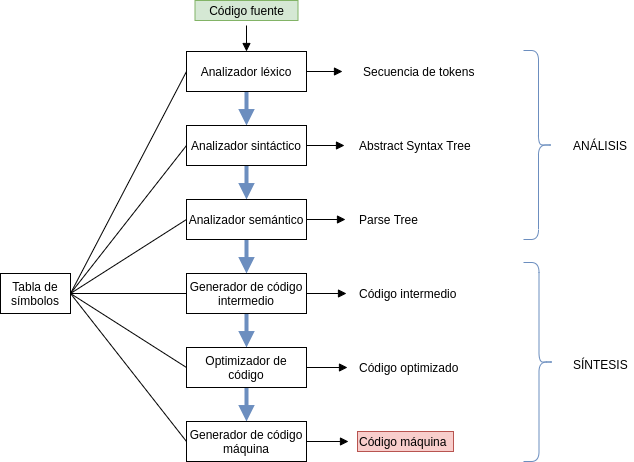
\includegraphics[scale=0.5]{fases_comp}
                \caption{Fases de compilación (Fuente: (Modificado) Compilers: principles, techniques, \& tools, \cite{aho_compilers:_2007}) }
                \label{fig:fasesComp}
            \par
        \endgroup

    \end{figure}

    Las fases que componen un compilador \cite{aho_compilers:_2007} pueden verse en la Fig. ~\ref{fig:fasesComp}.

\subsubsection{Analizador léxico}

    El analizador léxico, también llamado \emph{scanner} o \emph{lexer}, es aquel que lee la secuencia de caracteres del código fuente y los agrupa en
    otras secuencias llamadas \textbf{lexemas}. Por cada lexema, el \emph{scanner} genera un \emph{token} de la forma:
    La Fig. ~\ref{fig:fasesEjemplo} muestra las entradas y salidas de la fase en la parte superior.

    \begin{equation}
    \label{eq:1}
    <nombre\text{-}token, valor\text{-}atributo>
    \end{equation}
    Siendo, 
    \begin{itemize}
        \setstretch{1}
        \item \textbf{nombre-token}: símbolos abstractos usados durante el análisis sintáctico.
        \item \textbf{valor-atributo}: puntero a una entrada en la tablas de símbolos.
    \end{itemize}

    \paragraph*{Tabla de símbolos}

    El compilador guarda los nombres de variables o nombres de funciones (que aparecen en el
    código fuente) en la \textbf{tabla de símbolos}. También, almacena atributos 
    varios de dicha variable,
    por ejemplo: tipo, \emph{scope}, argumentos, tipo de pasaje de argumentos, 
    tipo de retorno, etc.
    Luego, se realiza un mapeo de \emph{tokens} con sus respectivos nombres de la tabla.

\subsubsection{Analizador sintáctico}

    El analizador sintáctico, también llamado \emph{parser}, utiliza el primer componente de cada \emph{token} ($nombre\text{-}token$ en ecuación ~\ref{eq:1}) para crear una representación en
    forma de árbol que muestre la estructura de los \emph{tokens}. Se genera un  \textbf{árbol sintáctico}. La Fig. ~\ref{fig:fasesEjemplo} refleja un esquema de esta fase en la parte superior.


\subsubsection{Analizador semántico}

    El analizador semántico emplea el árbol sintáctico y la tabla de símbolos (creada por el \emph{scanner}) para revisar la
    consistencia semántica del código fuente con respecto a la definición del lenguaje. También se realizan conversiones de un tipo de dato a otro (llamadas coerciones).
    Ver Fig. ~\ref{fig:fasesEjemplo} en la fase correspondiente.


\subsubsection{Generador de código intermedio}

    El generador intermedio tiene como meta producir código de tipo intermedio para obtener un lenguaje flexible y optimizable para la
    parte \emph{backend} del compilador. Observar dentro de la Fig. ~\ref{fig:fasesEjemplo} para una ilustración de la fase.

    El código intermedio puede tener muchas formas distintas (dependiendo de cada compilador).

\paragraph*{Propiedades de todo código intermedio}

Todo código intermedio debe cumplir las propiedades de:

    \begin{enumerate*}[label=\itshape\alph*\upshape)]
        \item ser fácil de generar;
        \item ser fácil de traducir a lenguaje máquina
    \end{enumerate*}

\paragraph*{Código de tres direcciones}

    Es una forma de código intermedio que consiste en una secuencia de instrucciones
    cuasi-\emph{assembler} con tres operandos por cada instrucción (cómo máximo). Cada
    operando puede actuar como un registro.

    Algunas características de este tipo de código son:

    \begin{itemize}
        \item Las instrucciones deben tener como máximo un \textbf{único operador} (órden de
        operaciones)
        \item El compilador debe generar un \textbf{nombre temporal} para guardar el valor retornado
        por la instrucción de tres direcciones (variables temporales tienen nombre).
    \end{itemize}


\subsubsection{Optimizador de código intermedio}

    El optimizador de código intermedio realiza mejoras sobre  dicho código para obtener un “mejor código” como salida de
    cada sucesiva optimización. Se presenta también una ilustración en la parte inferior de la Fig. ~\ref{fig:fasesEjemplo}.

    \begin{center}
        Mejor código = más rápido, más corto o de menor consumo de potencia.
    \end{center}

\subsubsection{Generador de código final}

    El generador de código final utiliza el código optimizado para generar el código final deseado.
    Si el lenguaje final es código máquina, se eligen los registros o lugares de memoria para
    cada variable usada en el programa. 
    En este trabajo, el código final buscado es código máquina. Por ello, se empleará el término "generador de código máquina".
    En este caso, se traducen instrucciones inmediatas a secuencias de instrucciones máquina.
    La parte inferior de la Fig. ~\ref{fig:fasesEjemplo} muestra una ilustración sobre esta fase.

    \begin{figure}[p]
        \begingroup
            \centering
                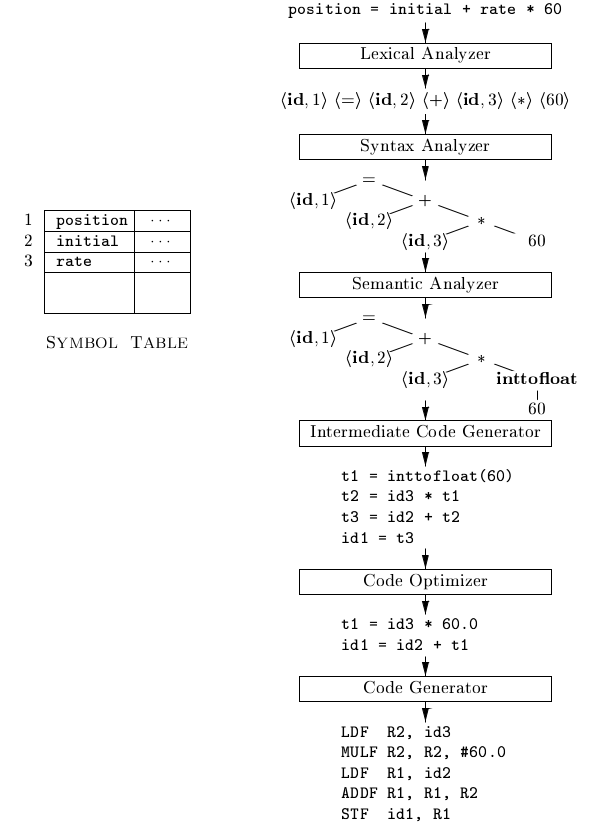
\includegraphics[width=0.8\textwidth,height=0.8\textheight,keepaspectratio]{ejemplo_fasescomp}
                \caption{Ejemplo completo de fases de compilación (Fuente: Compilers: principles, techniques, \& tools, \cite{aho_compilers:_2007}) }
                \label{fig:fasesEjemplo}
            \par
        \endgroup
    \end{figure}

\subsubsection{Instrucciones de compilación}

    \begin{lstlisting}[label=comandoC, caption= Comando de compilación del archivo \texttt{ejemplo.c} \cite{repo_trabajo_codigofuente} para GCC., language=bash]
        $ gcc -fdump-tree-original-raw -fdump-tree-all-graph -fdump-tree-gimple -da -S ejemplo.c 
        $ gcc -o ejemplogcc ejemplo.c \end{lstlisting}    

        %--------------------------------------------------------------------------------------------------------------------------
        % CAPITULO N: DESCRIPCION DEL MODELO EXPERIMENTAL (OPCIONAL)
        %--------------------------------------------------------------------------------------------------------------------------
        \chapter{Descripción del modelo experimental}

ES UN CAPITULO OPCIONAL

Puede formar parte del último Capítulo o en un Capítulo aparte. 
Se describe el modelo terminado, su funcionalidad, operación, manual de instrucciones, mediciones, etc.
    
        
        %--------------------------------------------------------------------------------------------------------------------------
        % CAPITULO N: RESULTADOS
        %--------------------------------------------------------------------------------------------------------------------------
        \chapter{Resultados}

Aquí se describen los resultados obtenidos luego de todo el proceso a modo de resumen haciendo 
referencia a lo desarrollado anteriormente. 

Los Resultados no deben incluirse en un Capítulo, es un apartado individual.    

        %--------------------------------------------------------------------------------------------------------------------------
        % CAPITULO N: CONCLUSIONES
        %--------------------------------------------------------------------------------------------------------------------------
        \chapter{Conclusiones }

Las Conclusiones deben tener una redacción clara, concreta y directa. No son un resumen del trabajo.
Deben reflejar los alcances y las limitaciones del estudio, recomendaciones, indicaciones de posible continuidad del trabajo, etc.
Se sugieren incluir los aspectos siguientes:

\begin{itemize}
    \setstretch{1}
    \item Resultados obtenidos en relación a la Solicitud de Aprobación de Tema.
    \item Conclusión General.
    \item Aporte que hace a la Ingeniería o a un campo de conocimiento. 
\end{itemize}

Las Conclusiones no deben incluirse en un último Capítulo, es un apartado individual 



        % ----------------------
        % --------- BIBLIOGRAFÍA
        % ----------------------

        \begingroup     

            \nocite{*}                      % Imprimir todas las bibliografias y referencias, aunque no se hayan citado

            \setlength\bibitemsep{1.5pt}    % 1.5pt interlineado entre entradas
            \setstretch{1}                  % 1pt interlineado entre lineas

            \printbibliography[type=book, title=Bibliografía]
            \printbibliography[nottype=book, title=Referencias]

        \endgroup

        % ----------------------
        % --------- ANEXO
        % ----------------------

        \begin{appendices} 

            \renewcommand{\thechapter}{\Roman{chapter}}         % Numeracion de los anexos en numeros romanos

            %--------------------------------------------------------------------------------------------------------------------------
            % ANEXO 1: TITULO ANEXO 1 
            %--------------------------------------------------------------------------------------------------------------------------
            \chapter{Hello}

Puede haber varios Anexos, numerar e iniciar cada uno en hoja nueva

Todo material complementario se ordena en los anexos, según el tipo de material pueden utilizarse varios anexos. 
Ejemplos: 
Hojas de datos. Desarrollos complejos que se llevan al anexo para simplificar la lectura del 
cuerpo del trabajo. Procedimientos complementarios que son se incidencia directa en el trabajo. 
Líneas de código que no se incluyen en el texto para no complicar la lectura (si el código es 
extenso debe incluirse en un archivo en el DVD

     

            %--------------------------------------------------------------------------------------------------------------------------
            % ANEXO 2: TITULO ANEXO 2 
            %--------------------------------------------------------------------------------------------------------------------------
            \chapter{Hola}

 
    
        \end{appendices}


    \backmatter

\end{document}